This appendix expands on the empirical application of Section~\ref{sec:application}. We display the recovered Stage-2 partial-correlation network with bank-level labels, summarize the recovered degree-centrality and region-pair structure, and discuss how the picture relates to the dynamic-marginal connectedness ranking of \textcite{demirer2018estimating}.

\subsection{Recovered network}

Figure~\ref{fig:ddly-network} shows the recovered Stage-2 network at the calibrated configuration $\lambda = 0.5$, $r_0 = 0.2$. Nodes are coloured by region; sovereign bond nodes are drawn larger than bank nodes. Bank labels are restricted to the ten most central banks (by Stage-2 degree); all ten sovereign bonds are labelled. The graph has $647$ edges among $\binom{106}{2} = 5{,}565$ possible pairs ($11.6\%$ density) and forms a single connected component.

\begin{figure}[H]
    \centering
    \begin{adjustbox}{center}
    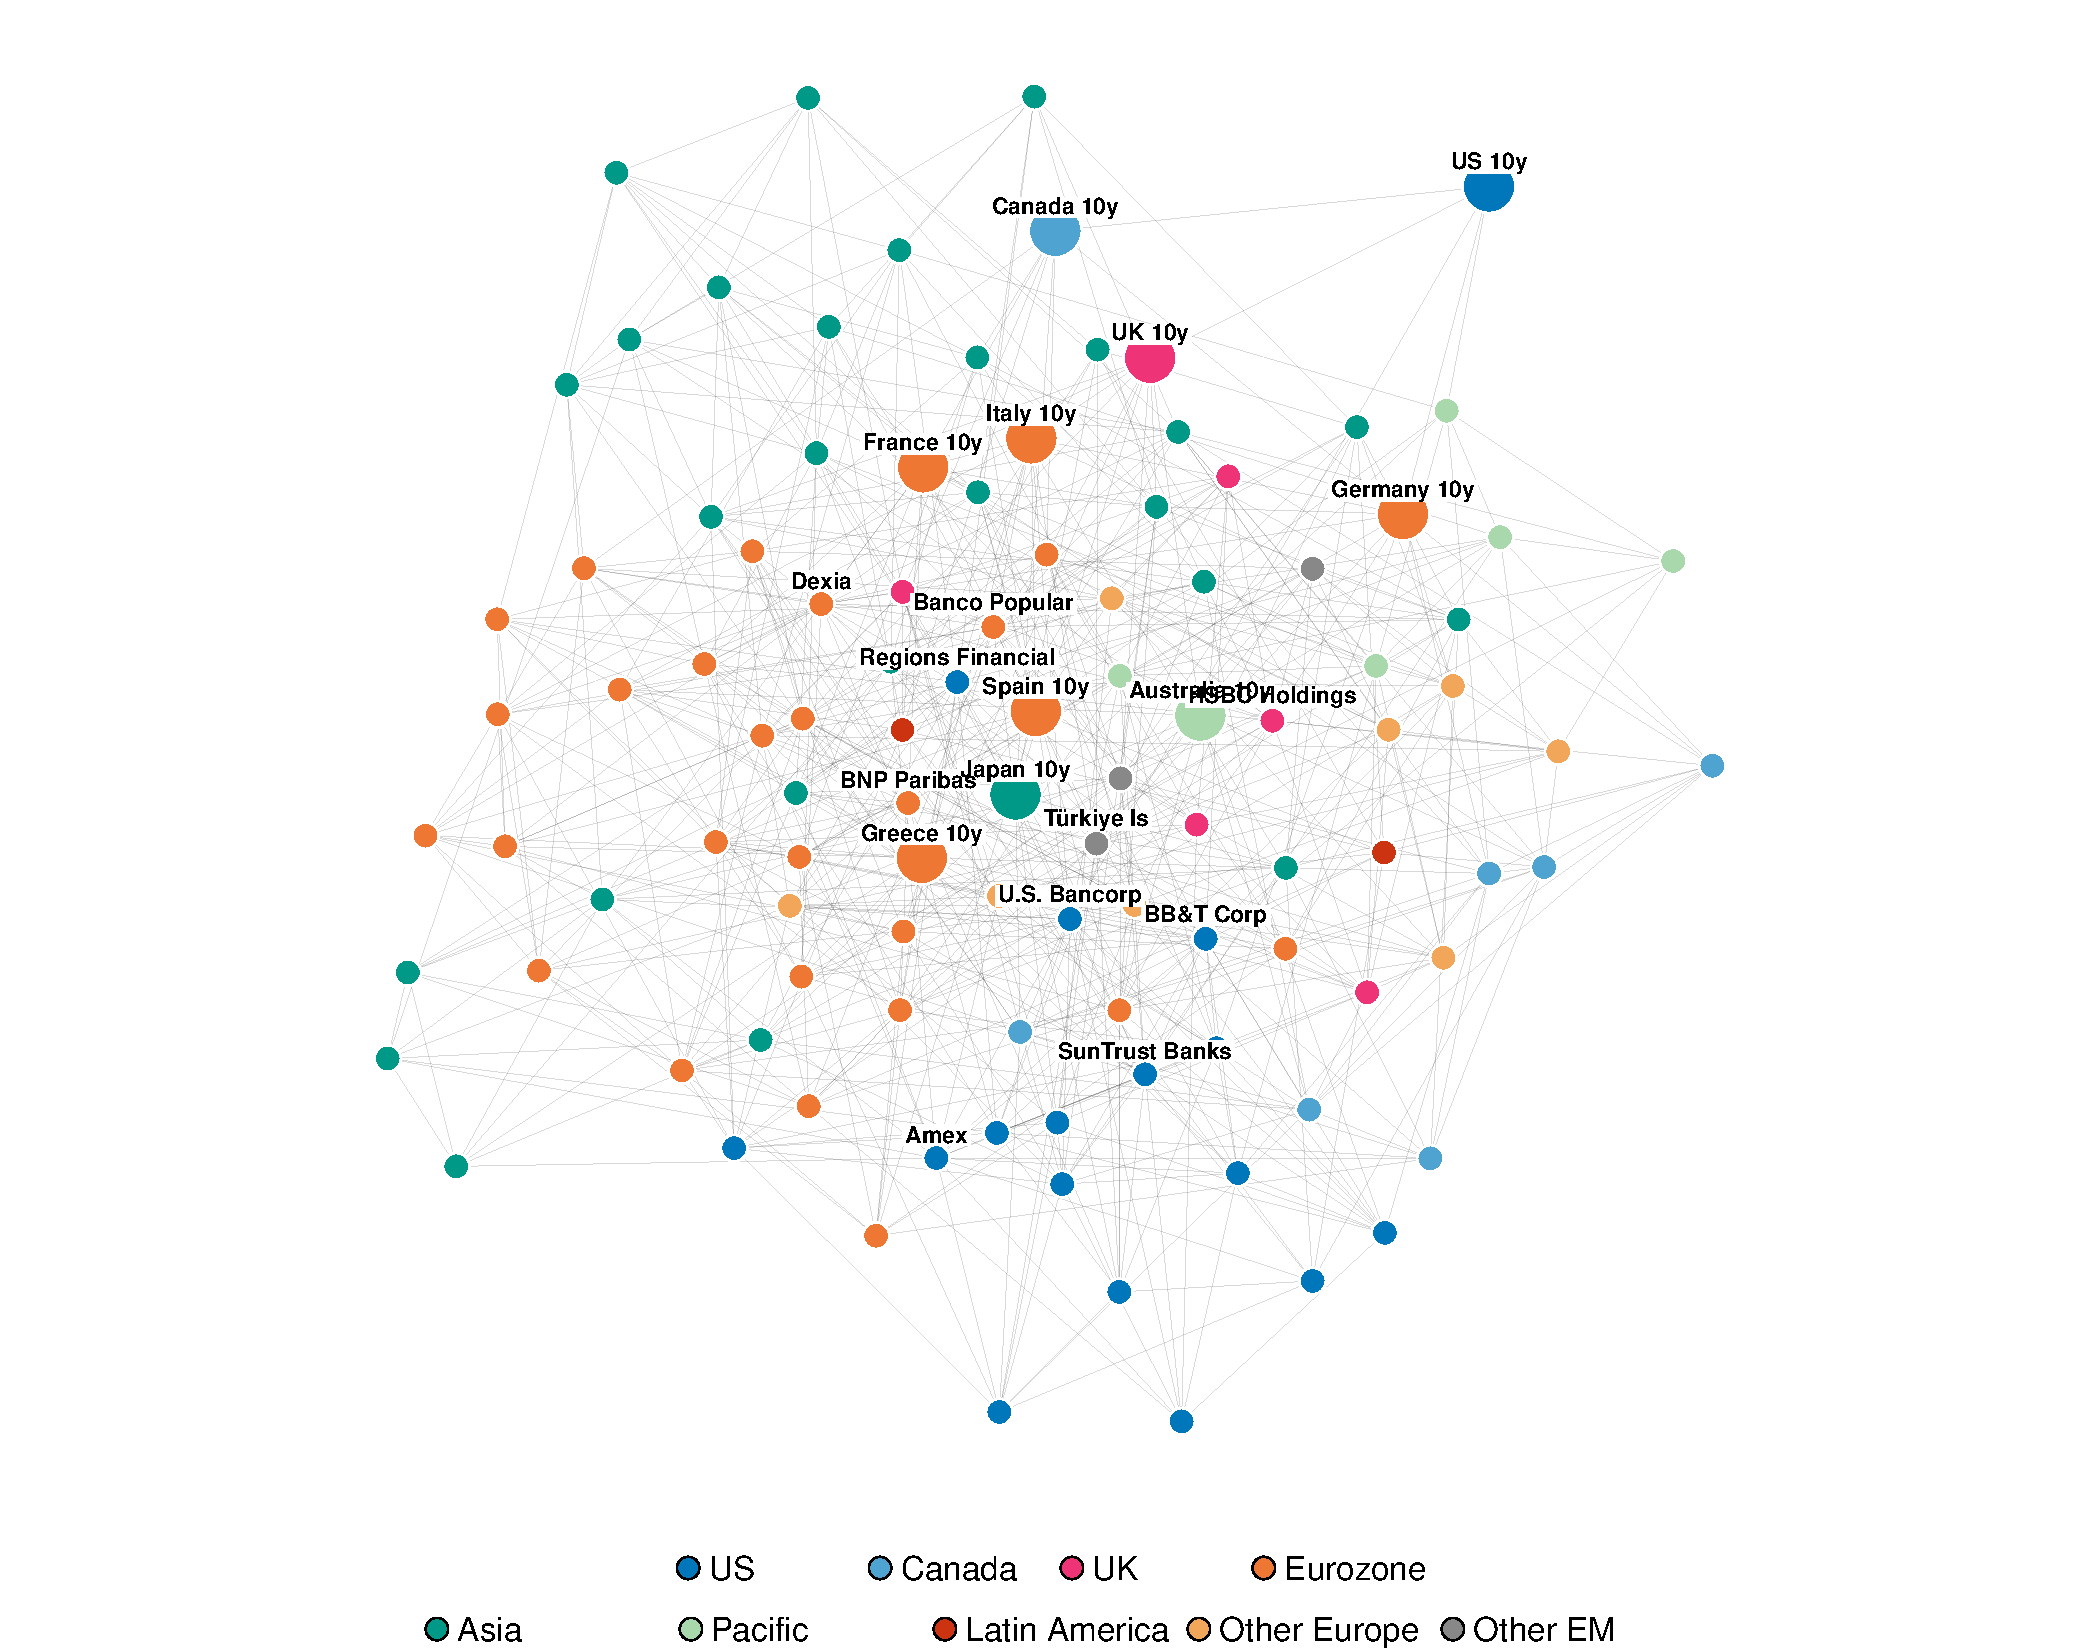
\includegraphics[width=1.2\textwidth]{../../2_analysis/output/figures/ddly_network_full_lambda0.50.pdf}
    \end{adjustbox}
    \caption{Recovered Stage-2 partial-correlation network on the full $p = 106$ DDLY panel. Edges are pairs with Stage-2 posterior inclusion probability above $0.5$. Bank labels show the ten most central institutions by Stage-2 degree; all ten sovereign bond nodes (drawn larger) are labelled. Layout: Fruchterman--Reingold.}
    \label{fig:ddly-network}
\end{figure}

\subsection{Top centrality and regional structure}

Table~\ref{tab:ddly-top-central} reports the ten banks with the highest Stage-2 degree centrality. The list is dominated by US regional banks (five entries: U.S.\ Bancorp, BB\&T Corp, Regions Financial, American Express, SunTrust Banks), Eurozone universals (three entries: BNP Paribas, Dexia, Banco Popular Espanol), one UK universal (HSBC Holdings), and one Other-EM representative (Turkiye Is Bankasi).

\begin{table}[H]
    \centering
    \caption{Top-10 banks by Stage-2 degree centrality on the $p = 106$ DDLY panel. Sovereign bonds excluded from the ranking.}
    \label{tab:ddly-top-central}
    % Auto-generated from ddly_results_full_lambda0.50.rds (r0=0.2 rerun).
% Top-10 banks (sovereign bonds excluded) by Stage-2 degree centrality.
\begin{tabular}{rlcr}
\toprule
Rank & Bank & Region & Degree \\
\midrule
1 & BNP Paribas & Eurozone & 20 \\
2 & Turkiye Is Bankasi & Other EM & 20 \\
3 & U.S. Bancorp & US & 19 \\
4 & Dexia & Eurozone & 18 \\
5 & BB\&T Corp & US & 18 \\
6 & Regions Financial & US & 18 \\
7 & HSBC Holdings & UK & 17 \\
8 & Banco Popular Espanol & Eurozone & 17 \\
9 & American Express & US & 17 \\
10 & SunTrust Banks & US & 16 \\
\bottomrule
\end{tabular}

\end{table}

The strongest within-region pair is intra-Eurozone, with $104$ edges linking Eurozone banks and the five Eurozone sovereigns (Germany, France, Italy, Spain, Greece). Asia ($85$ edges) and the US ($53$) are the next densest within-region clusters; the dominant cross-region bridges are Asia--Eurozone ($46$), Eurozone--US ($35$), and Asia--US ($26$). The Greek sovereign bond attains the highest sovereign-bond degree centrality ($17$), followed by France and Japan ($13$ each); Italy ($11$) and Spain ($10$) round out the top of the sovereign list. Most sovereign-bond connections in the recovered graph run to bank stocks rather than to other sovereigns; the comparison with \textcite{demirer2018estimating} below discusses this asymmetry.

\subsection{Comparison with \textcite{demirer2018estimating}}

\textcite{demirer2018estimating} estimate connectedness in the same global bank panel using a LASSO-VAR forecast error variance decomposition, and rank the most systemically connected banks by ``to-degree'' (the share of forecast-error variance other institutions explain through the focal one). Our object is a different one: we estimate the contemporaneous conditional-dependence graph implied by the precision matrix of log range volatilities, so the two estimands are not mechanically equivalent. Their measure is dynamic and marginal; ours is contemporaneous and conditional. Edges in our graph reflect joint movement after partialling out all other institutions in the panel, while their connectedness reflects predictive contributions over a short forecast horizon.

Two divergences from \textcite{demirer2018estimating} are worth flagging. First, they report that all $15$ of their top-ranked banks by net forecast-error connectedness carry the GSIB designation. Of our top $10$, only BNP Paribas and HSBC Holdings appear on the GSIB list. The remaining slots are predominantly US regional banks (U.S.\ Bancorp, BB\&T Corp, Regions Financial, American Express, SunTrust Banks), with one Belgian--French universal (Dexia), one Spanish universal (Banco Popular Espanol), and one Other-EM representative (Turkiye Is Bankasi). The bulge-bracket and Japanese megabanks DDLY single out as central, including JPMorgan Chase, Goldman Sachs, Mitsubishi UFJ, Mizuho, and Sumitomo Mitsui, rank between $30$ and $90$ in our partial-correlation degree. The pattern follows from the methodological difference. A bank whose log-volatility co-moves with many similar institutions after partialling out the rest of the panel will have high partial-correlation degree, while a bank that transmits idiosyncratic shocks to many counterparties will have high forecast-error connectedness. US regional banks form a tight cluster of similar institutions and dominate our list; bulge-bracket institutions transmit shocks across regions and dominate theirs.

The second divergence concerns sovereign bonds. \textcite{demirer2018estimating} report that sovereign bonds cluster among themselves and remain distinct from the national bank clusters. In our recovered graph, eight of the ten sovereign bonds have more bank neighbors than bond neighbors. The Greek $10$-year bond connects to two other sovereigns (Italy and Spain) and to fifteen banks across multiple regions. The same methodological asymmetry explains this. Partial correlation captures comovement that survives conditioning on every other variable in the panel, which can pull sovereign bonds toward bank stocks if their volatilities share common conditioning factors. Forecast-error variance decomposition captures the share of forecast-error variance one variable explains for another, which can keep bonds and banks in separate clusters even when their volatilities are correlated.

\subsection{Diagnostic reading}

Section~\ref{sec:application} reports that $94\%$ of Stage-2's added edges break the decomposability of the Stage-1 graph if injected there, and the Stage-2 graph contains $3{,}742$ induced chordless 4-cycles. Read together with Figure~\ref{fig:ddly-network}, the picture is one of a richly inter-connected global bank network whose structure cannot be described by a decomposable graph. The asymptotic guarantees of Theorem~\ref{thm:concentration} apply to the Stage-1 estimate $\hat G_D$ but do not transfer cleanly to the Stage-2 estimate $\hat G$. The recovered network is therefore appropriate as a descriptive object and as a misspecification diagnostic for the decomposable family, but qualitative claims about specific edges should be read in that light.\footnote{An empirical illustration of this caveat: re-running Stage 2 with $r_0 = 0.5$ instead of the calibrated $r_0 = 0.2$ leaves the diagnostic verdict unchanged (Stage-2 is non-decomposable, with chord-breaking rate $93.0\%$ vs $93.6\%$ and thousands of induced chordless 4-cycles in both runs) but produces a substantially different top-10 by degree centrality and shifts most region-pair counts by $5$--$40\%$. The diagnostic verdict is robust to the prior; the specific Stage-2 structure is not.}
